
\chapter{Laufzeitsicht}

\section{Szenario I}
\textbf{Anschalten der Roboter-Software}\\

\begin{figure}[h]
    \centering
    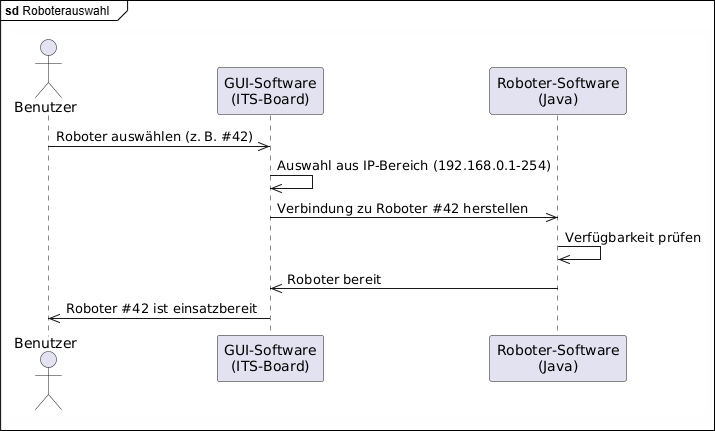
\includegraphics[width=0.8\linewidth]{diagrams/Roboterauswahl.png}
    \caption{Auswahl des Roboters}
    \label{fig:Auswahl}
\end{figure}

\clearpage
\section{Szenario II}
\textbf{Steuerbefehl über GUI-Software an einen ausgewählten, verfügbaren Roboter}\\

\begin{figure}[h]  
    \centering
    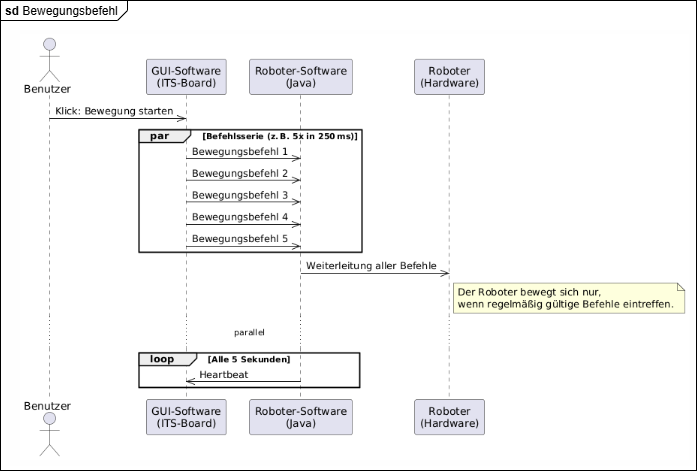
\includegraphics[width=0.8\linewidth]{diagrams/Bewegungsbefehl.png}
    \caption{Bewegungsbefehl über GUI}
    \label{fig:Bewegungsbefehl}
\end{figure}

\clearpage
\section{Szenario III}
\textbf{Fehlerfall: Verbindung zu Roboter fällt aus}\\

\begin{figure}[h]  
    \centering
    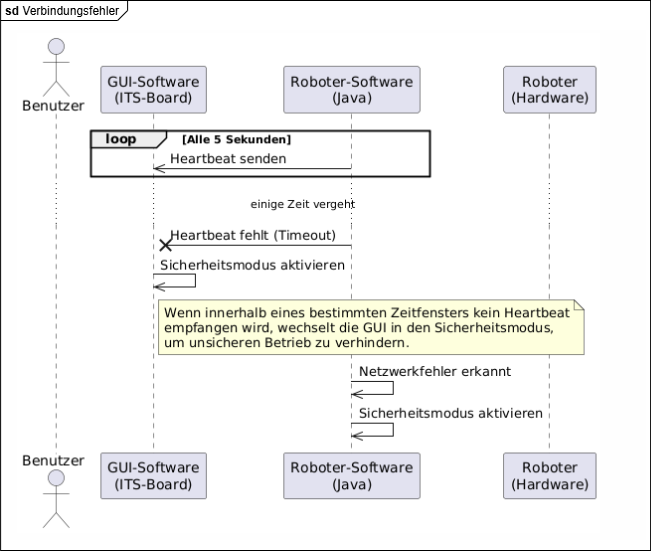
\includegraphics[width=0.8\linewidth]{diagrams/Verbindungsverlust.png}
    \caption{Verbindungsverlust}
    \label{fig:Verbindungsverlust}
\end{figure}



